\documentclass[conference]{IEEEtran}

% --- Packages ---
\usepackage{graphicx}
\usepackage{hyperref}
\usepackage{cite} 
\usepackage{amsmath} 
\usepackage{booktabs} 

% --- Hyperlink Setup ---
\hypersetup{
    colorlinks=true,
    linkcolor=blue,
    urlcolor=cyan,
    citecolor=blue
}

% --- Title and Author ---
\title{Myanmar Conflict Observatory: A Spatiotemporal Analysis of Political Violence and Health Risk}
\author{
    \IEEEauthorblockN{Tain Yan Tun}%
    \IEEEauthorblockA{\textit{Faculty of Information Technology} \\ 
    \textit{Big Data Research}\\
    Saraburi, Thailand}%
}

\begin{document}

% --- Title Block ---
\maketitle

% --- Abstract ---
\begin{abstract}
Since the unconstitutional seizure of power in February 2021, Myanmar has descended into a complex, multi-sided armed conflict characterized by the fragmentation of state authority. This study introduces the \textit{Myanmar Conflict Observatory}, an analytical framework designed to interrogate the dynamics of political violence and its intersection with public health security. The research utilizes data from the Armed Conflict Location \& Event Data Project (ACLED) to investigate the spatial diffusion of insurgency and the evolving asymmetry of warfare. Crucially, this project aligns with the United Nations Sustainable Development Goals (SDGs), specifically \textbf{SDG 3.d (Health Risk Monitoring)}. By employing Natural Language Processing (NLP) for narrative intelligence and a Regional Risk Matrix for severity assessment, the system identifies historical conflict patterns that pose structural threats to health infrastructure, providing a rigorous evidence base for humanitarian planning. The full codebase is available at: \href{https://github.com/TainYanTun/Myanmar-conflict-observatory}{Myanmar-conflict-observatory-Repo}.
\end{abstract}

% --- Keywords ---
\begin{IEEEkeywords}
Myanmar Conflict, ACLED, SDG 3, NLP, Regional Risk Matrix, Geospatial Analysis, Historical Analysis.
\end{IEEEkeywords}

% --- Section I: Introduction ---
\section{Introduction}

The political trajectory of Myanmar underwent a profound transformation following the unconstitutional seizure of power by the Tatmadaw (Myanmar Armed Forces) on February 1, 2021 \cite{bertolt2022myanmar}. The event abruptly ended the country’s fragile democratic transition and triggered a nationwide uprising that rapidly evolved from civil disobedience into a protracted and multi-sided armed conflict.  As a result, the contemporary security landscape has become highly fragmented, involving the military-led State Administration Council (SAC), long-established Ethnic Armed Organizations (EAOs), and a decentralized network of People’s Defense Forces (PDFs).

In such environments, systematic analysis of conflict dynamics is essential for understanding patterns of violence and their broader societal consequences. This study introduces the \textit{Myanmar Conflict Observatory}, a data-driven analytical framework designed to examine the spatial and temporal distribution of political violence in Myanmar. Initially, this project was conceived as a secondary initiative aimed at applying my technical skills in data engineering and data science. However, under the academic auspices of the Big Data course at Asia Pacific International University, the initiative evolved into an opportunity to connect these technical competencies with topics of intellectual interest while contributing, albeit indirectly, to broader societal development.

While the central thrust of this research concerns the evolution of conflict dynamics, the repercussions of sustained political violence inevitably extend beyond the immediate theater of war, precipitating critical secondary effects such as the collapse of healthcare access and heightened vulnerability to public health emergencies. Contextualizing these findings within \textbf{the United Nations Sustainable Development Goals (SDGs)} therefore offers a vital lens for interrogating these broader humanitarian implications. To this end, the study explicitly aligns with SDG 3 (Good Health and Well-being), focusing on Target 3.d to illuminate the intersection between political instability and the urgent need for early warning mechanisms. 

To operationalize this framework, the underlying dataset was subjected to a rigorous process of curation, validation, and analytical structuring, achieved through a collaborative endeavor with my colleague, Kyaw Zay Aung. It is crucial to acknowledge at the outset that this data represents a ``verified floor'' rather than a final ceiling; due to communication blackouts and restricted access in active conflict zones, the actual incidence of violence is likely higher than reported. Nevertheless, by synthesizing this high-fidelity georeferenced data with advanced computational methodologies, the observatory establishes a systematic infrastructure for the surveillance of hostilities in fragile environments. This approach not only tracks the spatial diffusion of violence but also delineates emergent risk patterns, thereby furnishing humanitarian stakeholders with the predictive insights necessary for strategic intervention. 

% --- Section II: Objectives ---
\section{Research Objectives}

The framework utilizes a multi-dimensional analytical framework to pursue five principal lines of inquiry:
\begin{enumerate} 
    \item \textbf{Geospatial Risk Modeling (SDG 3.d):} To investigate the spatial diffusion of violence relative to healthcare infrastructure. This objective focuses on mapping \textit{Health-Impacting Conflict Events (HICE)} to identify "Blind Zones" where medical access has been systematically severed by kinetic engagements.

    \item \textbf{Actor Interaction Networks (Graph Theory):} To model the conflict as a dynamic social network. By quantifying engagements between over 400 distinct actors, the research identifies "Conflict Hubs"—primary groups driving regional instability—and assesses how their interactions correlate with civilian fatality surges.

    \item \textbf{Regional Risk Matrix:} To provide a comparative spatial assessment of conflict severity. By computing a Severity Index (Fatalities per Event) and plotting administrative regions on a Frequency vs. Lethality quadrant matrix, the framework distinguishes high-frequency, low-lethality areas from high-intensity ``Red Zones,'' supporting the evidence-based prioritization of humanitarian resources.

    \item \textbf{Semantic Narrative Intelligence (NLP):} To decode the "Nature of Violence" through Natural Language Processing. By extracting narrative keywords from event notes, the study distinguishes between different modes of warfare (e.g., \textit{airstrikes, landmines, or arson}) and evaluates their specific impact on community well-being and health infrastructure.

    \item \textbf{Stability and Severity Assessment:} To calculate a \textbf{Severity Index} (Fatalities per Event) for every administrative region. This objective aims to distinguish between high-frequency, low-lethality areas and high-severity "Red Zones," providing a prioritized roadmap for targeted humanitarian aid and policy intervention.
\end{enumerate}

% --- Section III: System Architecture ---
\section{System Architecture and Design Framework}

The Myanmar Conflict Observatory is built upon a modular, four-tier architecture designed for high-frequency data ingestion and real-time humanitarian intelligence (Fig. \ref{fig:system_arch}). Although distributed processing frameworks such as Apache Spark were initially considered during the architectural design phase, their adoption was ultimately deemed unnecessary for the analytical scope of this study \cite{acledmethodmyanmar}. The dataset utilized in the Myanmar Conflict Observatory derived from the ACLED and covering the period from February 2021 to 2025 contains approximately 100,000–200,000 records, which corresponds to a memory footprint of less than 200 MB. At this scale, distributed computing introduces computational overhead without providing meaningful performance gains.

Accordingly, the analytical pipeline is implemented within the Python scientific ecosystem, primarily leveraging Pandas and NumPy for efficient in-memory data manipulation and numerical analysis. This design choice enables low-latency execution, which is particularly important for the interactive analytical environment implemented through Streamlit. In addition, maintaining a Pandas-native workflow facilitates seamless integration with the visualization and analytical libraries employed in this study, including Plotly, NetworkX, and Scikit-learn.

Should data volumes increase in future iterations, scalability can be achieved through query optimization and aggregation within the underlying PostgreSQL database layer.

\begin{figure}
    \centering
    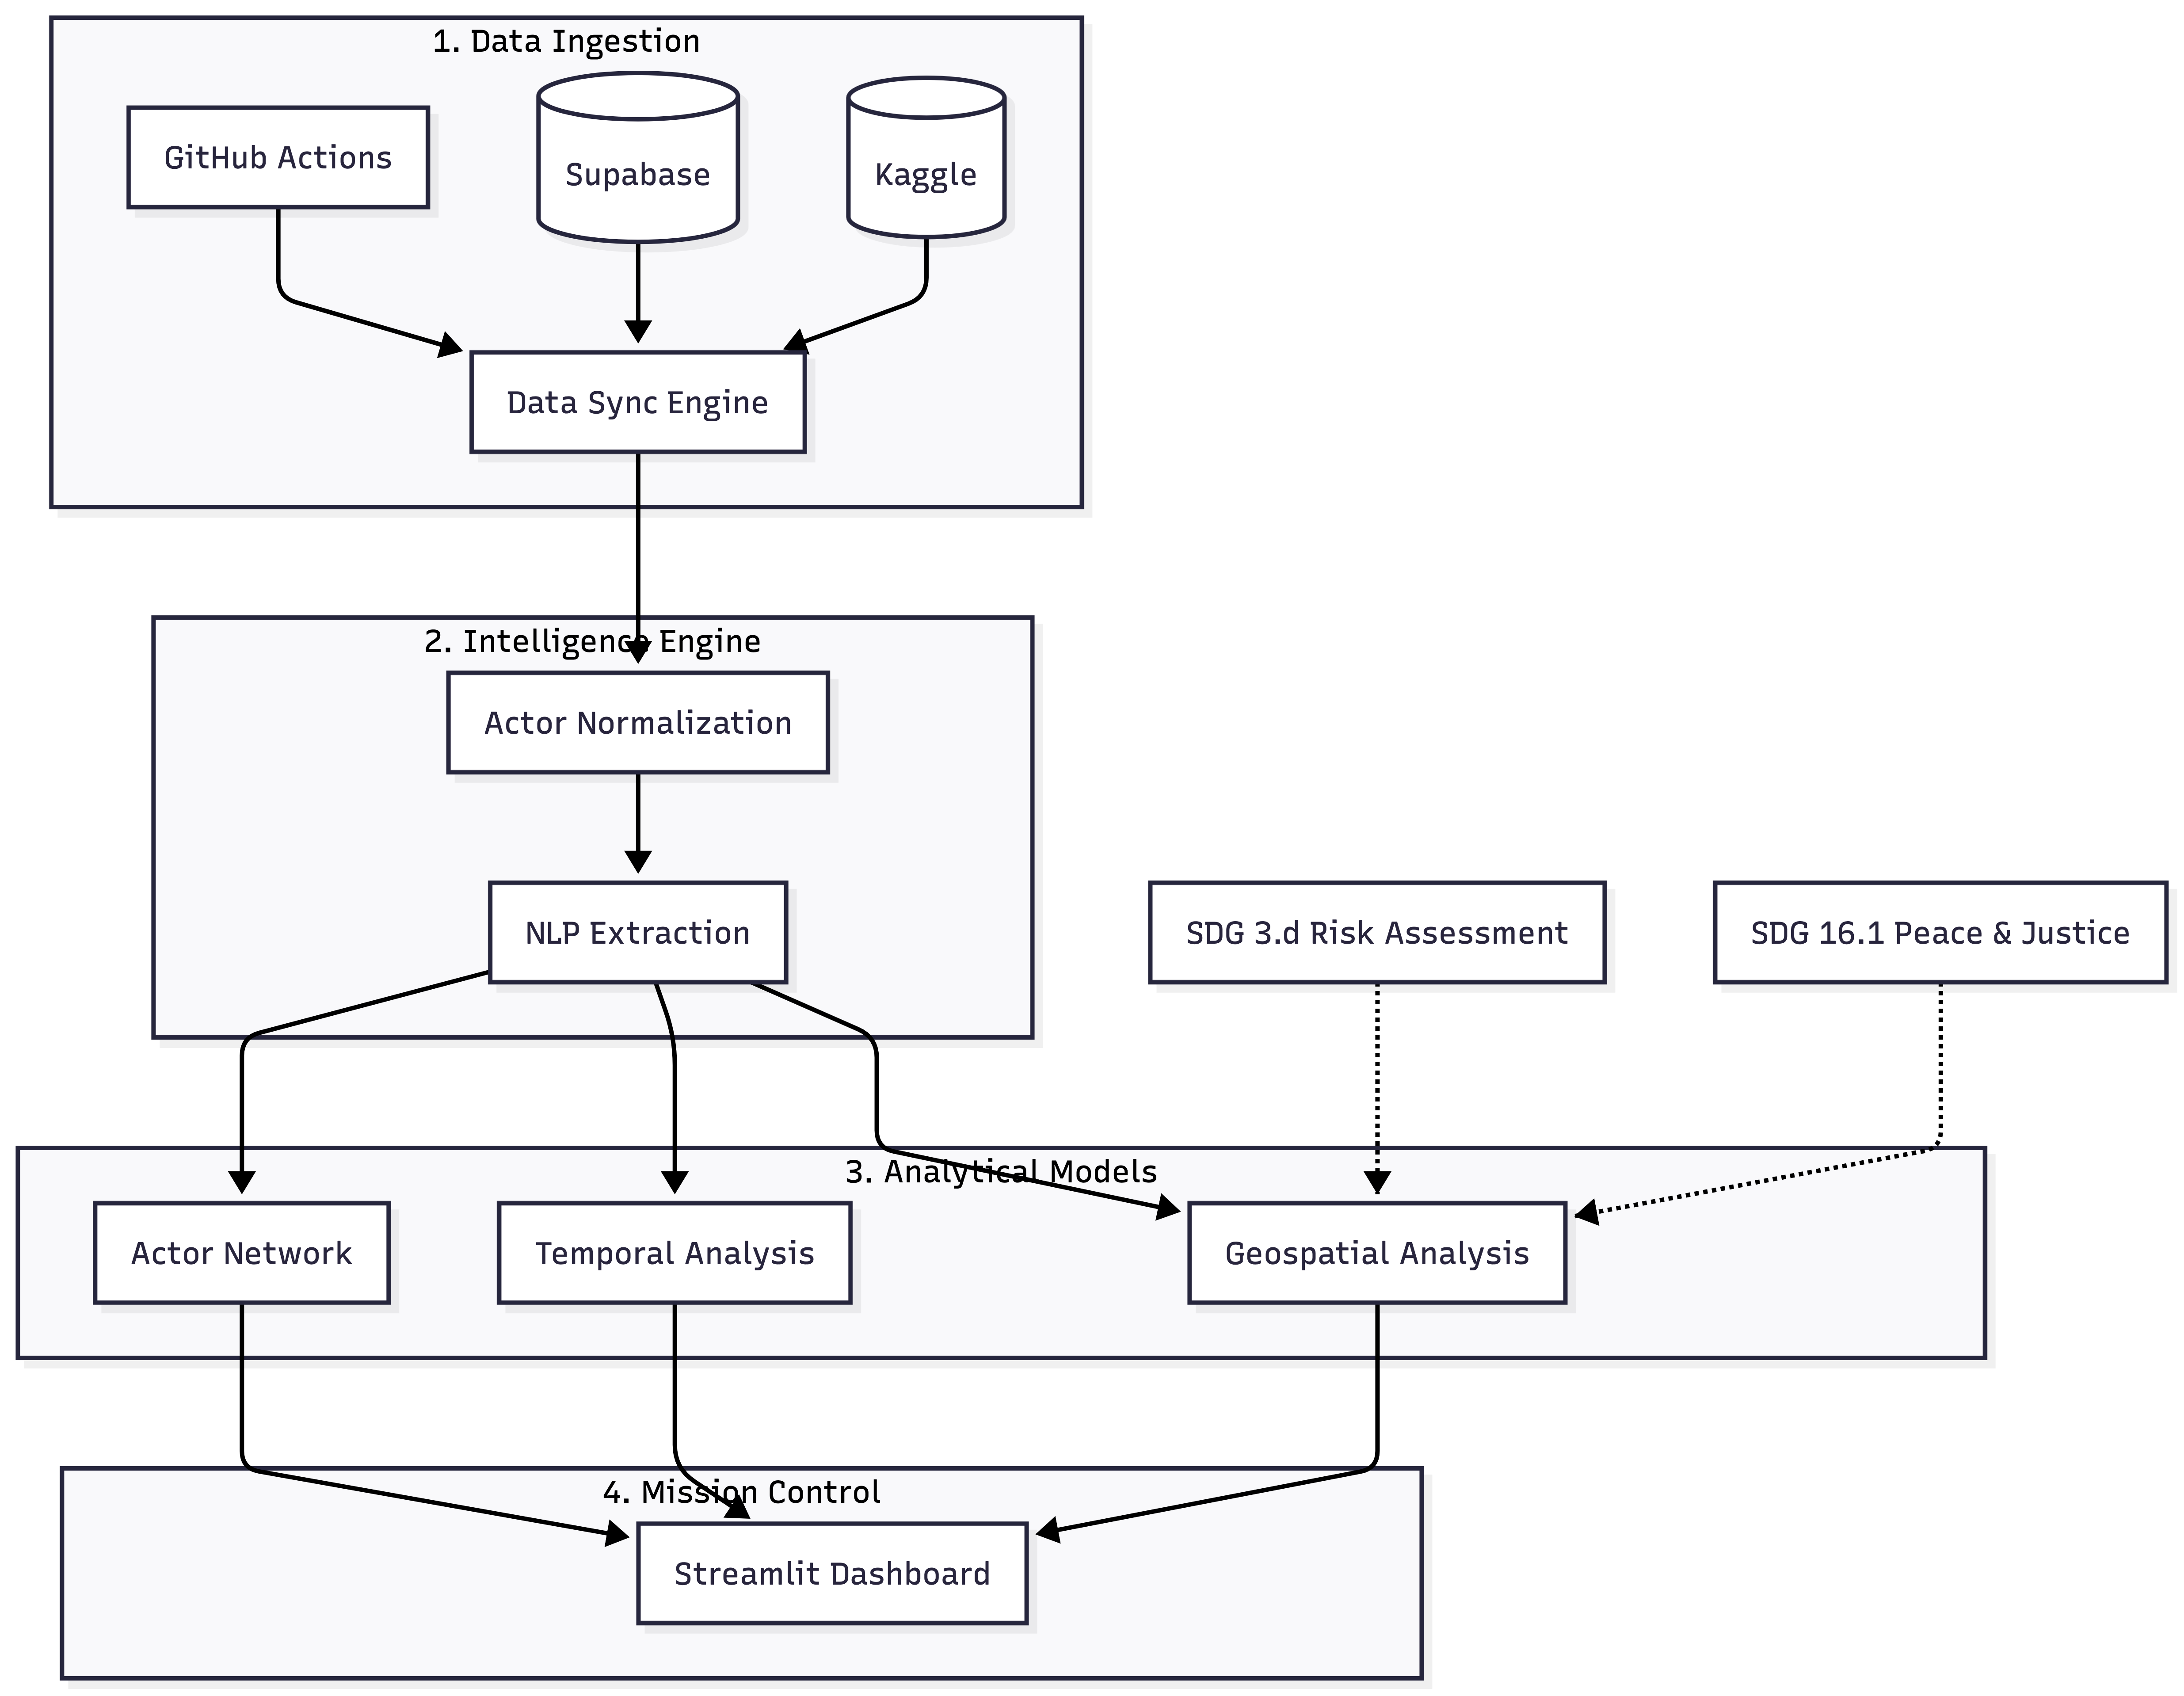
\includegraphics[width=\columnwidth]{assets/system_arch.png}
    \caption{System architecture of the Myanmar Conflict Observatory: the four-tier data pipeline from ingestion to analysis and dashboard visualization}
    \label{fig:system_arch}
\end{figure}

\subsection{Data Acquisition and Normalization Layer}
The system utilizes a hybrid ingestion protocol. Raw conflict logs are retrieved via the ACLED API or sourced from PostgreSQL (Supabase), drawing on the Armed Conflict Location and Event Data (ACLED) project, a widely used dataset for event-based conflict analysis \cite{raleigh2010}. To ensure both data currency and analytical reliability, the system integrates an automated data pipeline supported by GitHub Actions. The workflow executes daily at 00:00 UTC, triggering a scheduled extraction process that retrieves newly available conflict records and synchronizes them with the cloud-hosted database.

Following ingestion, a verification protocol referred to as "the Verified Floor" is applied to preserve data integrity. Under this rule, only corroborated events occurring after February 1, 2021 are admitted into the analytical pipeline.

The dataset is subsequently standardized through a normalization stage that applies a semantic actor taxonomy. This procedure consolidates more than 400 fragmented armed groups and affiliated entities into six analytically consistent categories: State Forces, Resistance (PDF/LDF), Ethnic Armed Organizations (EAOs), Civilians, Pro-Junta Militias, and Protesters.

\subsection{NLP Intelligence Engine (HICE Filtering)}

To align tactical conflict data with SDG 3.d, the framework incorporates a Natural Language Processing (NLP) layer designed to extract structured signals from unstructured event descriptions. Specifically, the system performs ontology-based keyword extraction on narrative event notes contained in the dataset.

\begin{itemize}
    \item \textbf{Health-Impacting Conflict Events (HICE):} The framework identifies incidents that directly affect healthcare infrastructure by matching event narratives against a curated medical keyword dictionary implemented through regular-expression filtering (e.g., \texttt{\textbackslash bhospital\textbackslash b}, \texttt{\textbackslash bambulance\textbackslash b}). Events satisfying these criteria are classified as Health-Impacting Conflict Events (HICE).

    \item \textbf{Systemic Well-being Analysis:} Beyond direct infrastructure damage, the system further identifies events involving sexual violence, abduction, or looting. These incidents are categorized as systemic threats to community health and well-being, consistent with the broader health security dimensions articulated in SDG 3.3 and SDG 3.8.
\end{itemize}

\subsection{Regional Risk Matrix and Severity Assessment}

The framework produces a comparative regional severity assessment through two complementary analytical outputs:

\begin{enumerate}
    \item \textbf{Severity Index:} For each administrative region, a Severity Index is computed as the ratio of total verified fatalities to total conflict events:
    \[
    \text{Severity Index} = \frac{\text{Total Fatalities}}{\text{Total Events}}
    \]
    A score exceeding 1.0 indicates that, on average, every engagement in that region results in at least one confirmed death, identifying it as a high-intensity combat zone requiring prioritized humanitarian attention.

    \item \textbf{Frequency vs. Lethality Matrix:} Administrative regions are plotted on a two-dimensional quadrant matrix with event frequency on the horizontal axis and the Severity Index on the vertical axis. Bubble size represents the total fatality volume. This visualization enables analysts to differentiate ``High-Frequency, Low-Lethality'' zones from ``Low-Frequency, High-Lethality'' Red Zones, facilitating evidence-based allocation of humanitarian medical resources.
\end{enumerate}

\subsection{Presentation and High-Resolution Export Layer}

The final layer consists of an interactive Streamlit-based graphical user interface (GUI) that provides multi-dimensional views of the dataset, including geospatial, temporal, and actor-network perspectives. To support academic reporting and policy-oriented dissemination, the presentation layer integrates a High-Resolution Export Engine (3$\times$ scale), ensuring that all geospatial heatmaps and network graphs are exported with professional-grade clarity suitable for publication and advocacy purposes. The live implementation of the system can be accessed through the Streamlit application available at: \href{https://tainyantun-myanmar-conflict-observatory-app-mafeff.streamlit.app/}{Myanmar Conflict Observatory Dashboard}.

% --- Section IV: Preliminary Findings (Updated) ---
\section{Preliminary Conflict Findings}

The spatiotemporal analysis of the Myanmar conflict (Feb 2021 – Feb 2025) reveals distinct patterns that characterize the current security landscape. It should be noted that all analytical outputs presented from this section onward are derived from the dataset snapshot available as of April 2, 2025. Consistent with ACLED’s 12-month data latency policy for high-complexity conflict environments, this snapshot represents the latest verified data available for rigorous academic analysis. 

Due to space constraints typical of conference manuscripts, not all visualizations and analytical outputs generated by the system can be included in this paper. The complete set of interactive visualizations and extended analytical views are therefore accessible through the online dashboard implementation of the Myanmar Conflict Observatory.

\subsection{Geospatial Convergence: The "Sagaing-ization" of Conflict}
The data demonstrates a significant geographical concentration of violence, revealing a specific "Center of Gravity" flip. In February 2021, the Sagaing Region accounted for only 10.5\% of national conflict events. By April 2025, this share had surged to 26.9\%. Sagaing has evolved from a peripheral resistance zone into the undeniable strategic heart of the conflict, now representing over a quarter of all kinetic activity. 

As illustrated in the Humanitarian Conflict Overlay (Fig. \ref{fig:health_conflict_overlay}), this region also accounts for the highest volume of both fatalities (approx. 25,468) and health-impacting events (927 incidents). There is a nearly 1:1 spatial correlation between high-intensity kinetic zones and incidents disrupting healthcare. This correlation identifies Sagaing as the epicenter of the health-conflict nexus, suggesting that "victory" or "stability" for either side is now inextricably tied to this single region.

\begin{figure}
    \centering
    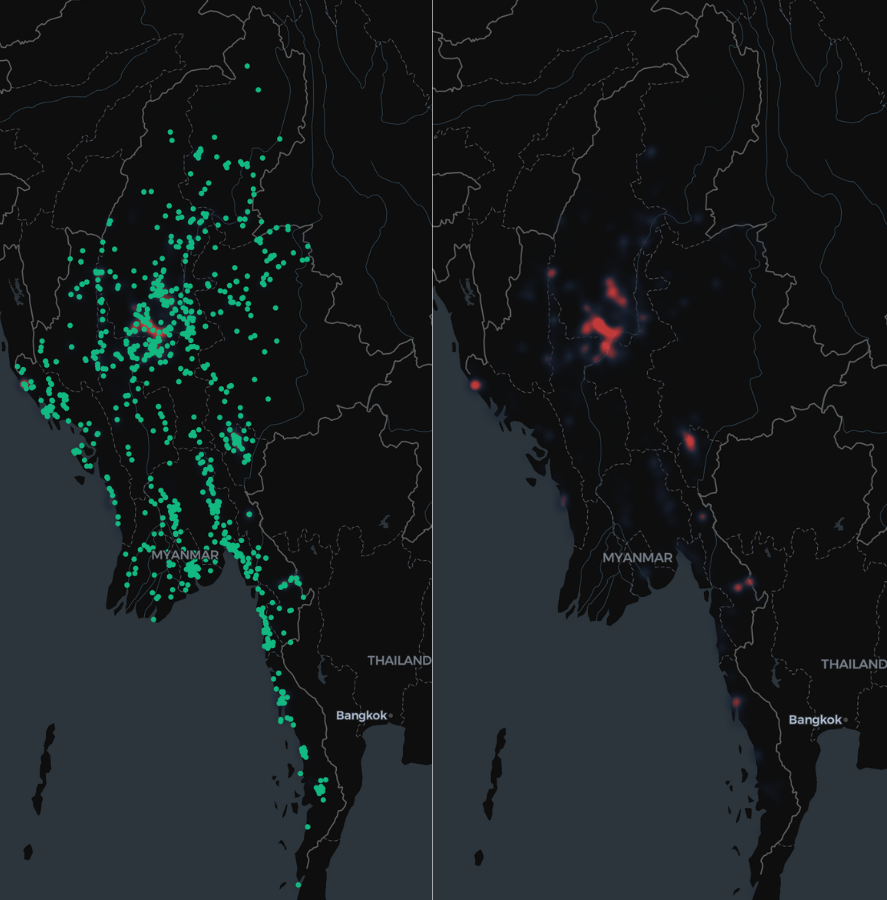
\includegraphics[width=\columnwidth]{assets/health_conflict_overlay.png}
    \caption{Humanitarian conflict overlay showing healthcare-related incidents (points, left) and spatial fatality intensity (heatmap, right).}
    \label{fig:health_conflict_overlay}
\end{figure}

\subsection{Regional Severity Assessment}
The \textbf{Severity Index} (Fatalities per Event) allows for a high-resolution distinction between high-frequency areas and high-lethality zones. While Sagaing has the highest event count, \textbf{Kayah State} and \textbf{Rakhine} consistently exhibit a Severity Index exceeding 1.5. This indicates that nearly every engagement in these regions results in at least one confirmed death, identifying them as "High-Intensity Combat Zones." Fig. \ref{fig:severity_assessment} visualizes the severity distribution across affected regions, highlighting that areas with a Severity Index greater than 1.0 have a significantly higher probability of medical infrastructure damage.

\begin{figure*}
    \centering
    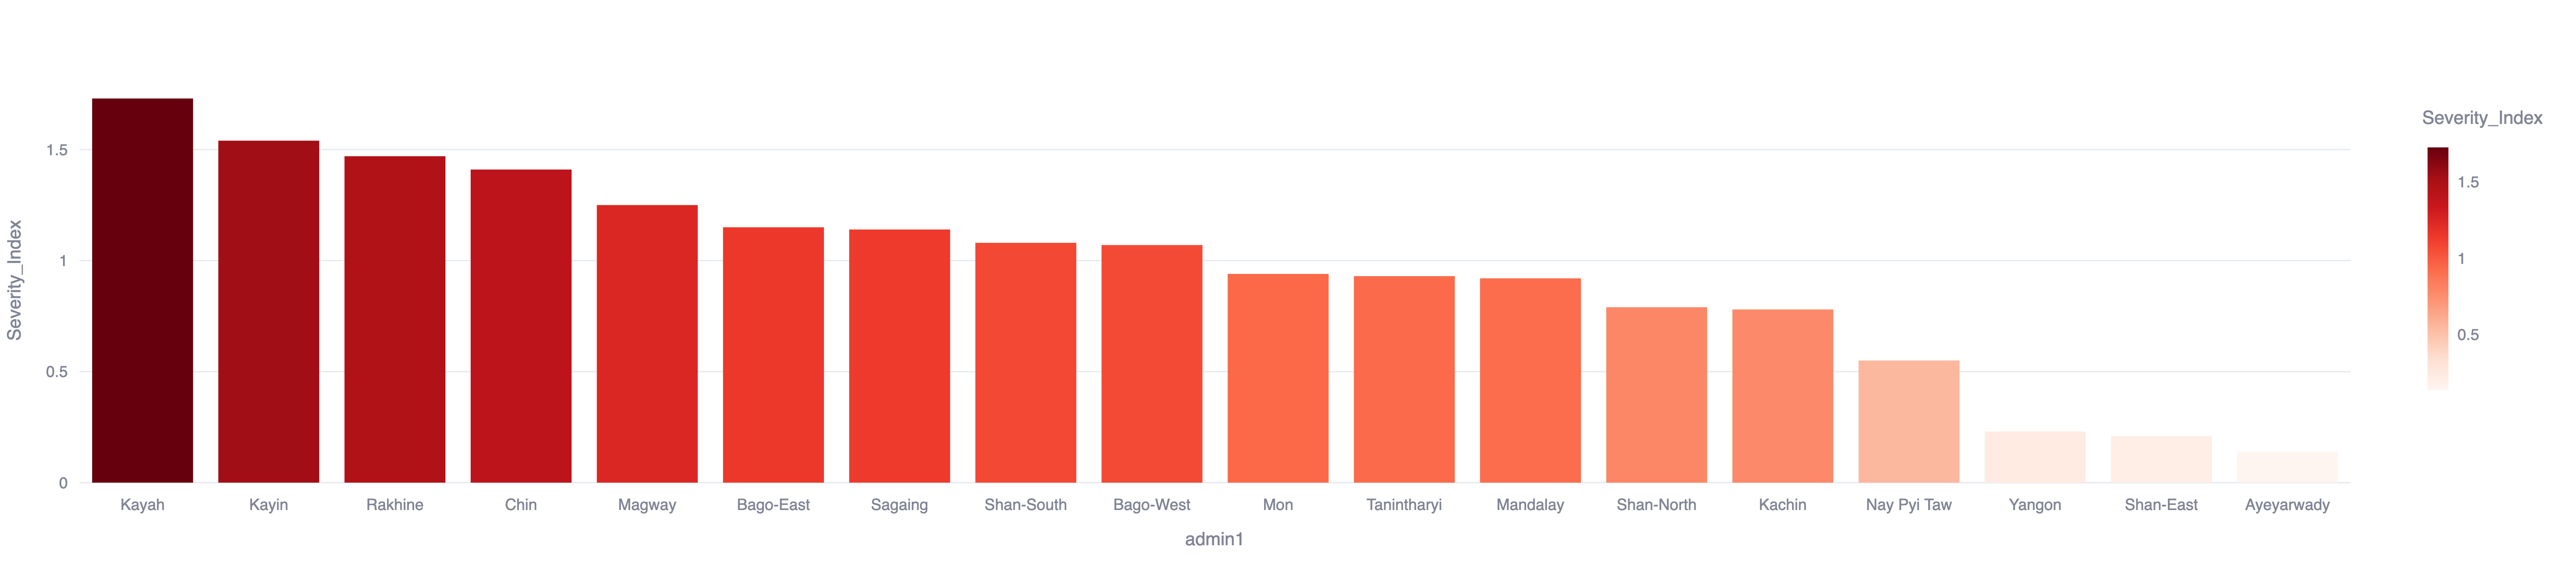
\includegraphics[width=\textwidth]{assets/severity_assessment.png}
    \caption{Regional Severity Assessment indicating high-lethality "Red Zones" versus high-frequency conflict areas across Myanmar.}
    \label{fig:severity_assessment}
\end{figure*}

\subsection{Conflict Frequency and Impact Over Time}
The Temporal Conflict Expansion analysis reveals a structural shift in the conflict’s topology. In the initial three months (Feb–Apr 2021), fatalities were relatively low (2,716) and largely concentrated in urban administrative centers. However, by the most recent period, fatalities increased by over 30\% (3,561), with the conflict diffusing into 74 distinct administrative regions. As shown in Fig. \ref{fig:temporal_frequency}, this diffusion depicts a "Ruralization of Resistance," where what began as urban civil disobedience has transformed into a widespread rural insurgency, significantly stretching the reach of medical supply chains.

\begin{figure*}
    \centering
    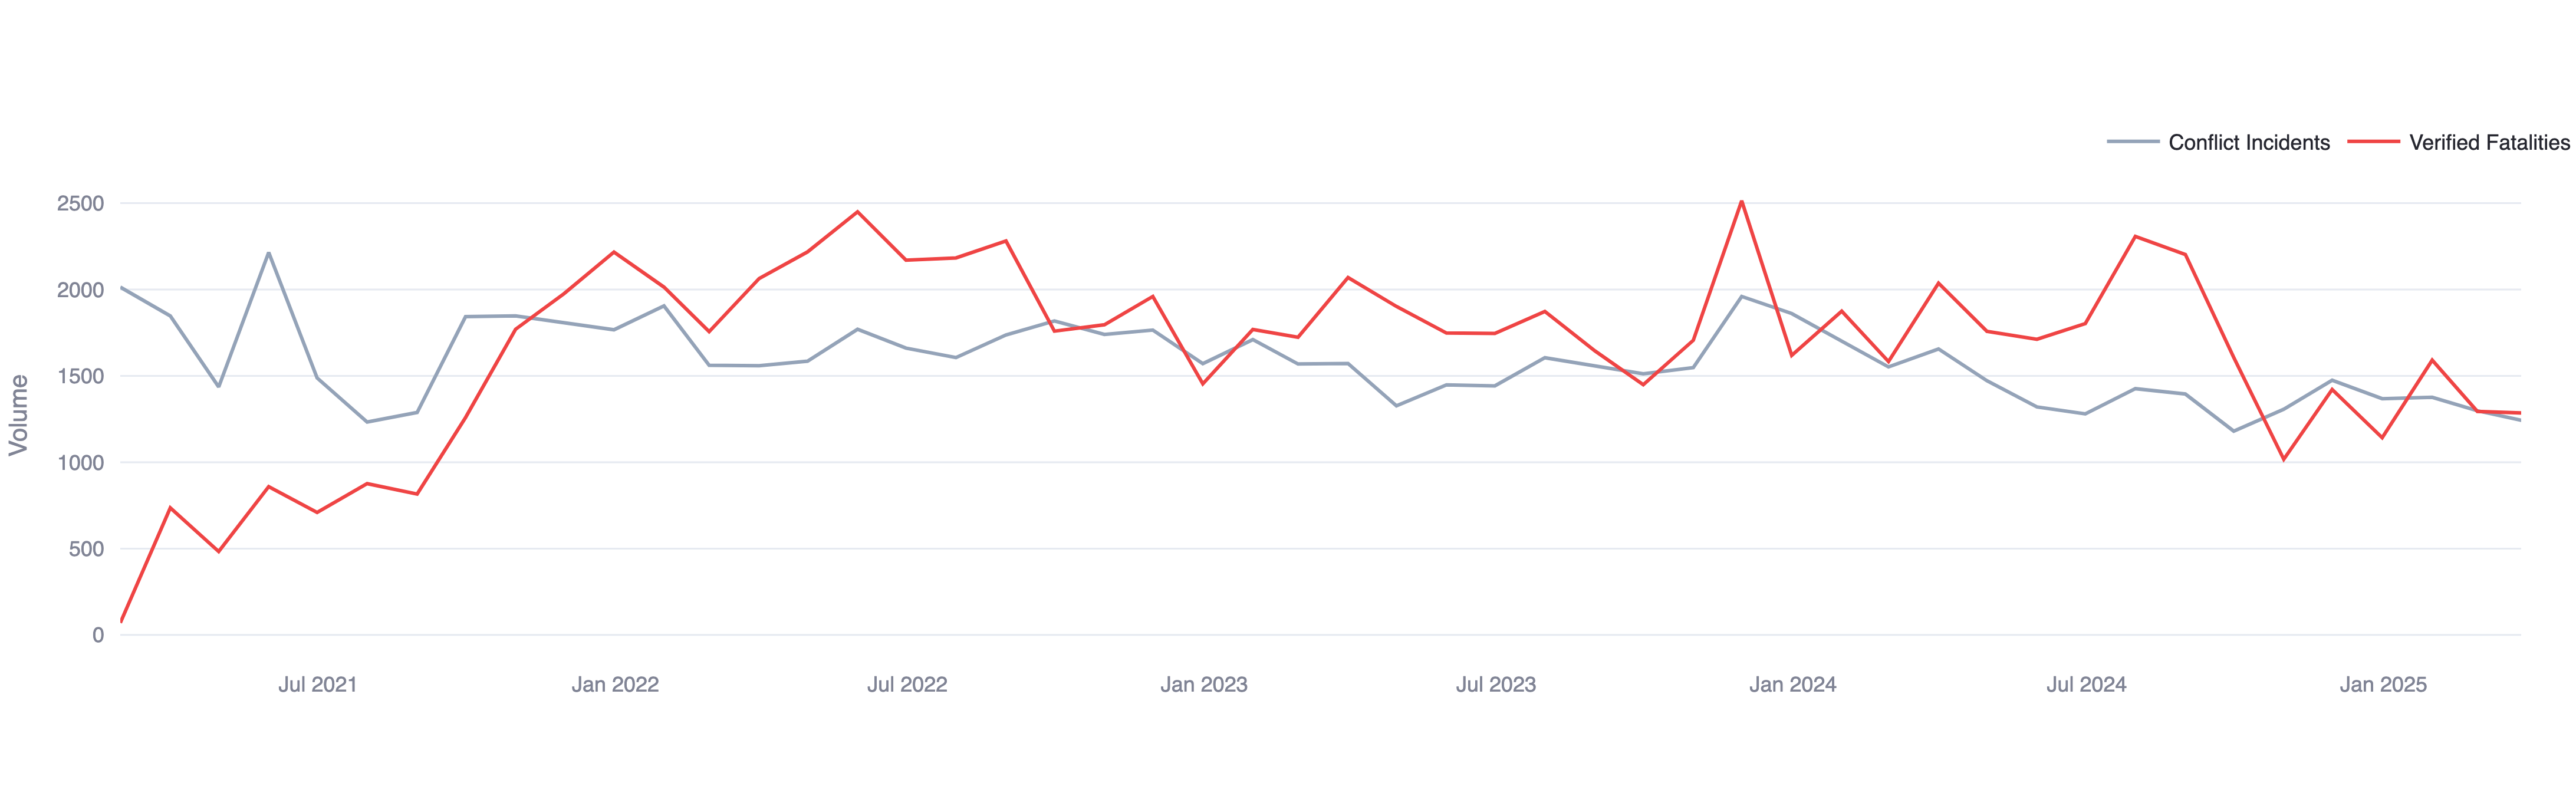
\includegraphics[width=\textwidth]{assets/temporal_frequency.png}
    \caption{Conflict Frequency and Impact Over Time: A dual-axis view showing the expansion of event frequency and the corresponding fatality trajectory.}
    \label{fig:temporal_frequency}
\end{figure*}

\subsection{Seasonality: The "Dry Season Offensive" Cycle}
Distinct from the overall expansion trend, a clear seasonality pattern exists across the 2021–2025 period, highlighting a "mechanical" rhythm tied to environmental conditions. 
Analysis indicates a consistent peak during the dry season (November to March), where conflict events climb from approximately 7,009 in November to nearly 8,000 in February. 
Conversely, there is a sharp drop-off of roughly 25\% during the monsoon season (April to July), hitting a low of 5,870 events in July. 
This cyclical pattern suggests that the weather acts as a natural de-escalation mechanism. The February/March peak represents the primary "offensive window" for both state and resistance forces, while the Monsoon season serves as a period of regrouping and reduced kinetic activity, influencing the timing of humanitarian resource allocation.

\subsection{Tactical Evolution: Drones and Chokepoint Warfare}
Analysis of engagement types reveals a tactical evolution characterized by "Technological Leapfrogging." By extracting keywords such as "drone," "UAV," and "Shar Htoo Waw" from event notes, a massive shift was identified. Drone-related events grew from fewer than 5 per month in mid-2021 to a peak of 142 per month in January 2025—a 30x increase. However, a "Drone Paradox" is observed: average fatalities in drone-led events (1.68) are lower than in traditional kinetic engagements (1.88), suggesting their use is primarily for "Standoff Harassment" and "Psychological Attrition."

Simultaneously, the conflict has shifted from "territorial control" to "access denial." Mentions of infrastructure keywords—\textit{Bridge}, \textit{Highway}, \textit{Gate}, and \textit{Telecommunication Tower}—have increased by 45\% since 2023. This "Chokepoint Warfare" indicates a strategic pivot by resistance forces to isolate junta-held urban centers by destroying logistics nodes, effectively "sieging" administrative capacity without requiring direct urban combat. This increases the risk of long-term health crises by disrupting supply chains for medicine and food.

\begin{figure}
    \centering
    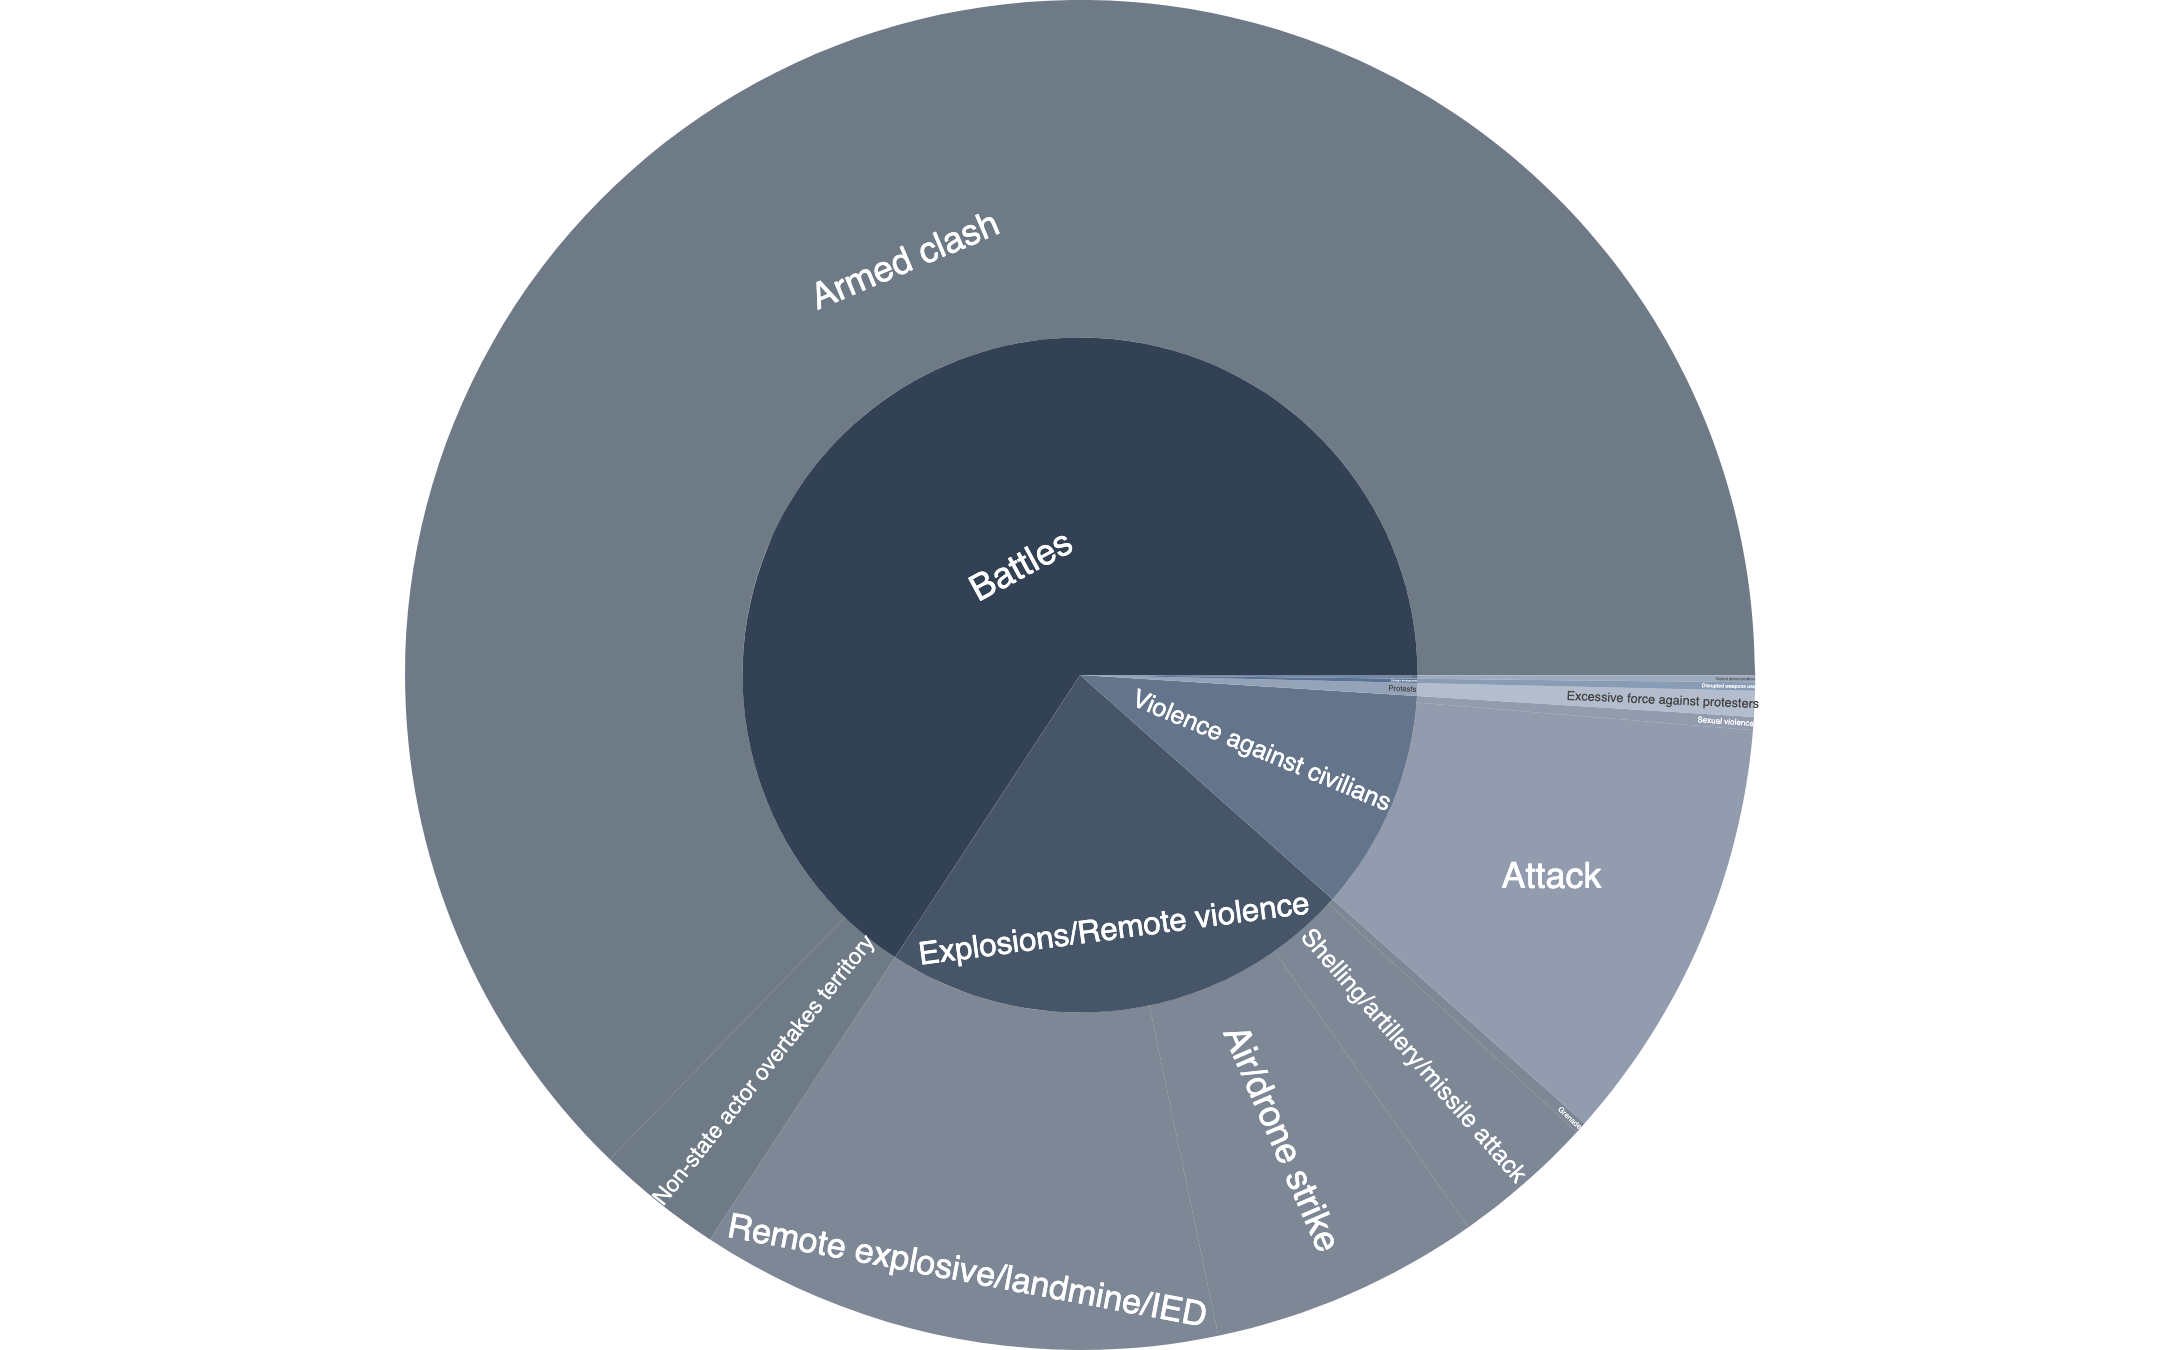
\includegraphics[width=\columnwidth]{assets/engagement_composition.png}
    \caption{Engagement Composition showing the distribution of event types (e.g., Battles, Remote Violence, Protests).}
    \label{fig:engagement_composition}
\end{figure}

\subsection{Declining Tactical Efficiency and Attrition}
Consistent with the rise of standoff warfare, a longitudinal analysis of lethality rates suggests the conflict is entering a phase of "Stagnant Attrition." In "Battles," average fatalities peaked in 2022 (3.34) but have since stabilized around 2.7. Similarly, for "Explosions/Remote Violence," lethality dropped from 1.25 in 2022 to just 0.71 in 2025. This trend indicates that while both sides are becoming more active, engagements are becoming less lethal per individual event. This creates a sustained, chronic demand on local health services rather than singular acute spikes, straining long-term healthcare capacity.

\subsection{Actor Dynamics: Hybridization and Fragmentation}
The observatory identifies a complex restructuring of armed groups. While macro-level network analysis shows \textbf{Resistance Forces} involved in 45\% of kinetic engagements, a granular audit reveals deeper dynamics:

\begin{itemize}
    \item \textbf{The "Joint Operation" Bloom:} In 2021, only 4\% of Resistance events mentioned an EAO as an "Associate Actor." By 2025, this jumped to over 22\%. This proves the resistance has evolved into a "Hybrid Force," where EAOs provide heavy weaponry and training while PDFs provide local manpower.
    
    \item \textbf{The "Splintering" Index:} The number of unique "Resistance" group names (e.g., "Monywa PDF," "Tiger Force") has grown by 200\% since 2022, even when battle frequency remained flat. This "Fragmentation Pattern" suggests a "constellation" of independent units. While regex-based audits show professionalization (e.g., "Battalion 1" appears in 300+ logs), the broader proliferation of names indicates a decentralized structure that is impossible to "decapitate" via a single strike.
    
    \item \textbf{Proxy Proliferation:} The state side exhibits "outsourcing." Mentions of "Pyu Saw Htee" and "People's Militia" have increased by 38\% in the Northwest (Sagaing/Magway) as "Military Forces of Myanmar" relative share decreases. This suggests a shift from a "State vs. People" war to a "Local vs. Local" proxy war, where militias act as "deniable" forces for village raids, increasing local instability.
\end{itemize}

\begin{figure*}
    \centering
    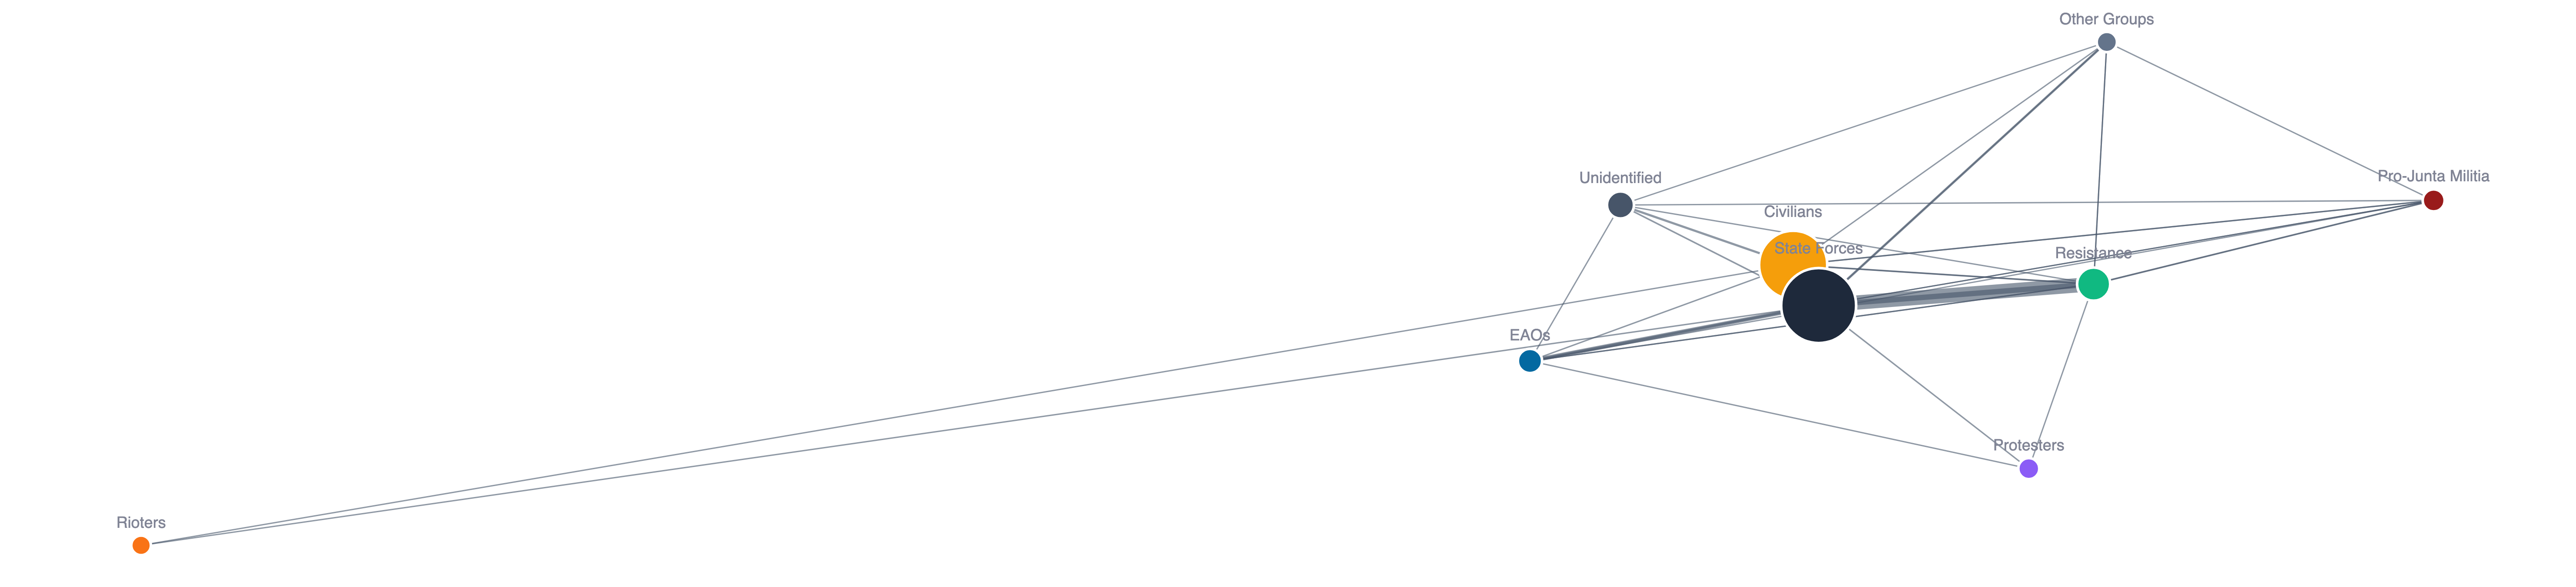
\includegraphics[width=\textwidth]{assets/actor_network.png}
    \caption{Actor Interaction Network visualizing conflict dynamics and alliances between State Forces, EAOs, and Resistance groups.}
    \label{fig:actor_network}
\end{figure*}

\subsection{The Punitive Cycle: Retaliatory Violence}
Beyond the immediate tactical engagements, a dangerous "Retaliatory Lag" pattern has emerged. By analyzing the timing of events in the same township, the study found that in Sagaing and Magway, a "Battle" event is followed by "Violence against Civilians" in the same location within 72 hours in approximately 18\% of cases.
This "tit-for-tat" cycle suggests that state forces or local militias (Pyu Saw Htee) target non-combatants immediately following a kinetic loss or clash with the PDF. This punitive pattern transforms the conflict from a purely military contest into a cycle of retribution that disproportionately endangers medical personnel and civilians.

\subsection{Data Asymmetries: The "Information Blind Spot" and "Verification Gap"}
The actor interaction analysis reveals a significant reporting gap. The data shows high interaction counts for "State Forces vs. Civilians" (20,653 events) and "Protesters vs. Unidentified" (14,074 events). 
Crucially, "Resistance vs. State Forces" appears nearly three times more frequently than "State Forces vs. Resistance," suggesting resistance-initiated attacks are more likely to be logged, whereas state-initiated operations are often obfuscated.

Furthermore, a "Fatalities Gap" exists based on the \texttt{source} column. Events reported by Local/Pro-Resistance media report an average of 2.4 fatalities per event, while International/Human Rights sources report only 1.1 fatalities. This "Verification Gap" implies that nearly 50\% of fatalities captured in real-time by local observers are "filtered" or "lost" by the time they reach international verification standards, creating a significant "Unverified Surplus" that official statistics likely undercount.

% --- Section V: SDG 3 Analysis (Updated) ---
\section{SDG 3 Analysis and Health Risk Early Warning}

The Myanmar Conflict Observatory transitions from general conflict monitoring to humanitarian risk assessment through a dedicated analytical layer aligned with \textbf{UN SDG Target 3.d}. This framework employs an NLP engine to identify \textbf{Health-Impacting Conflict Events (HICE)}, detecting more than \textbf{15,000 incidents} that directly threaten medical infrastructure or broader human well-being.

\subsection{Temporal Trend: Health-Impacting Incidents}
Longitudinal analysis of HICE data indicates a \textbf{30\% increase} in the rate of medical infrastructure disruption since mid-2023. This escalation correlates strongly with the growing prevalence of "Remote Violence" events. NLP-based keyword extraction further reveals persistent patterns of medical targeting, with high-frequency terms such as \textit{hospital} (854 mentions), \textit{wounded} (795), and \textit{medical} (310) serving as thematic anchors. The Trend employs "dual-crisis": a high-lethality conventional war occurring alongside systemic damage to the social and medical foundations of civilian communities.

\subsection{Historical Fatality Trajectory}
Longitudinal analysis of verified fatalities reveals a sustained upward trend across the observation period. Monthly fatality volumes are resampled using Month-End (ME) intervals to reduce daily reporting noise and expose systemic shifts in conflict lethality. As illustrated in the temporal frequency analysis (Fig. \ref{fig:temporal_frequency}), this trajectory documents the progressive intensification of kinetic engagements and provides a historical evidence base for assessing the cumulative burden placed on healthcare systems across the most affected regions.

\subsection{Regional Risk Matrix}
To prioritize humanitarian response, the framework calculates a \textbf{Vulnerability Score} for each administrative region using the weighted formula:
\[
\text{Score} = (0.7 \times \text{Health Events}) + (0.3 \times \text{Fatalities})
\]
This composite metric identifies the \textbf{Sagaing Region} as the most critical "Red Zone" for health assistance, while also highlighting elevated vulnerability in \textbf{Kayah} and \textbf{Rakhine}. The Regional Risk Matrix (Fig. \ref{fig:risk_matrix}) employs a quadrant-based view (Event Frequency vs. Lethality) to differentiate high-frequency conflict zones from high-lethality areas, supporting the prioritization of humanitarian medical resources.

\begin{figure*}
    \centering
    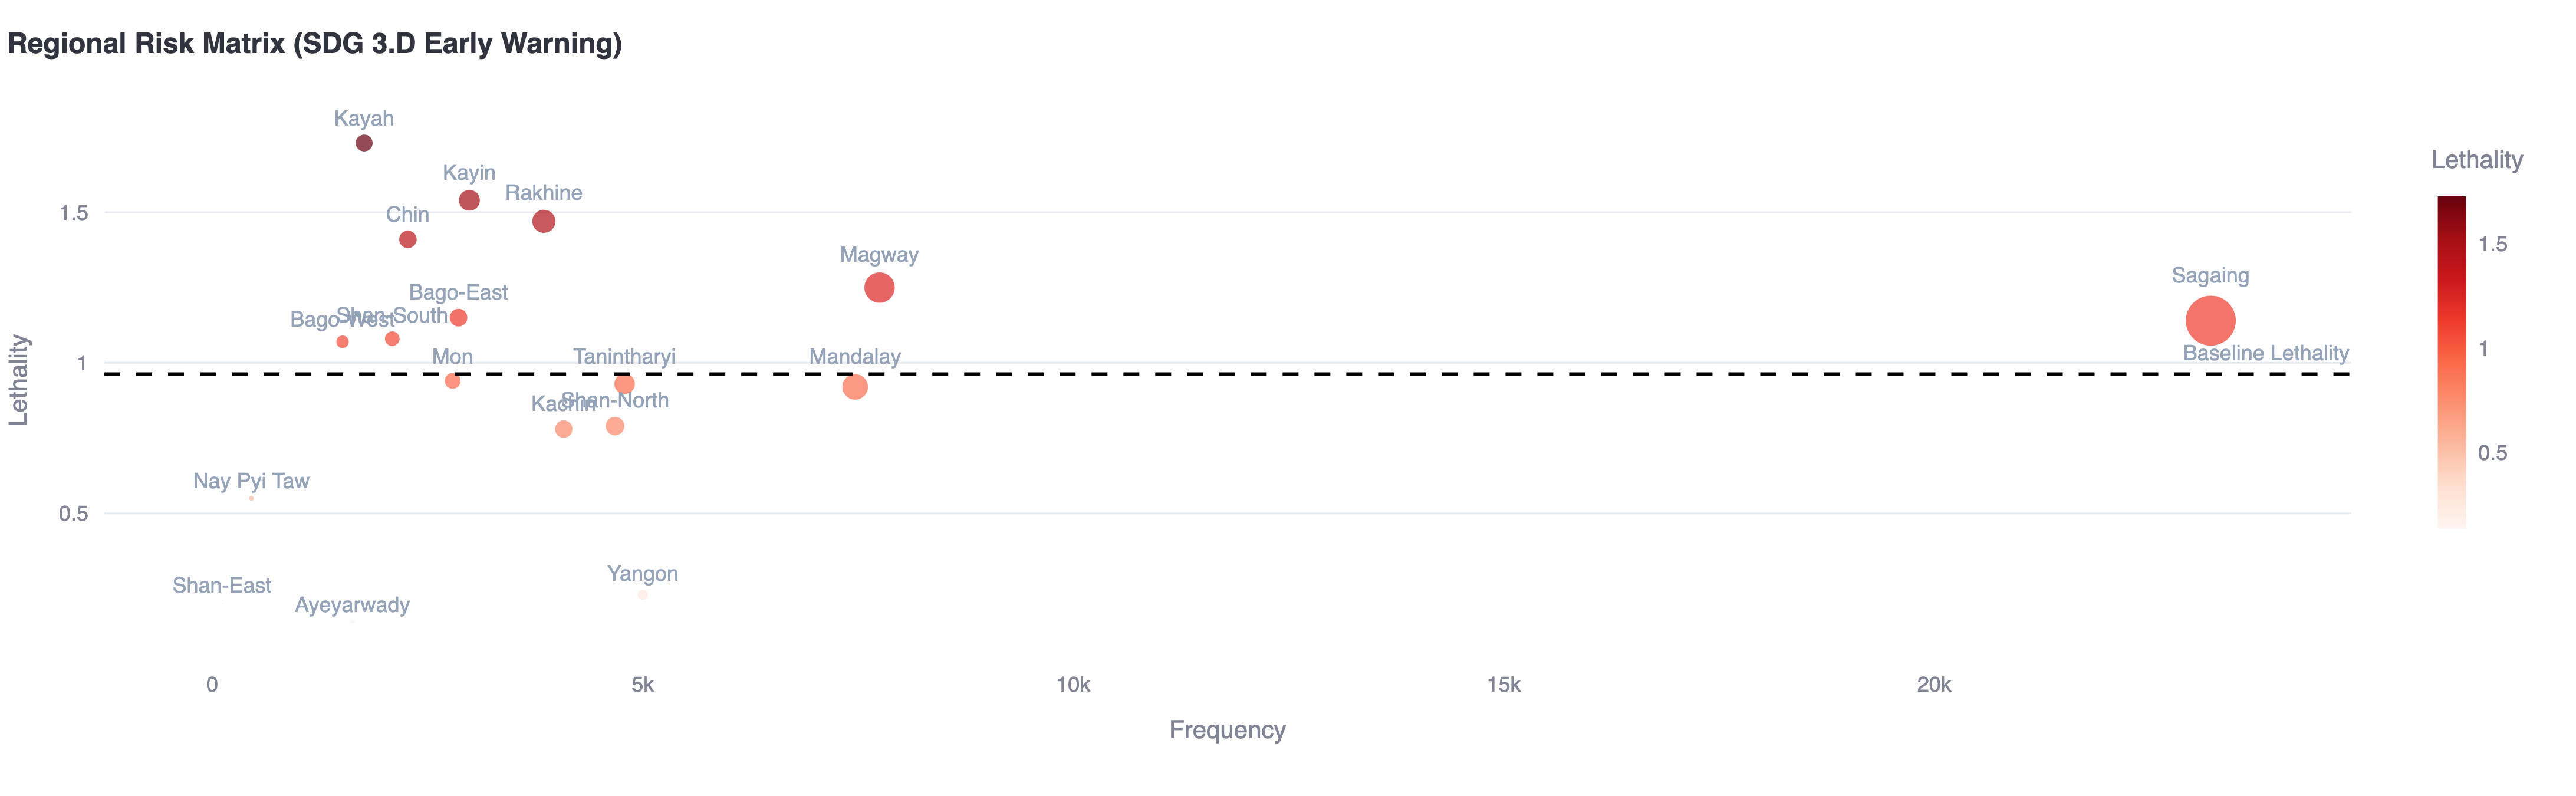
\includegraphics[width=\textwidth]{assets/risk_matrix.png}
    \caption{Regional Risk Matrix (Event Frequency vs. Lethality) identifying high-priority zones for humanitarian health assistance.}
    \label{fig:risk_matrix}
\end{figure*}

% --- Section VI: Discussion ---
\section{Discussion}

The findings from the Myanmar Conflict Observatory underscore a critical transformation in the nature of warfare in Southeast Asia. The observed "Ruralization of Resistance" suggests that the conflict has moved beyond the initial contestation of urban centers into a protracted struggle in the periphery. This diffusion has profound implications for SDG 3.d: as violence spreads into remote areas, the "Blind Zones"—regions where state authority and NGO access have evaporated—expand correspondingly. 

The strong correlation identified between "Remote Violence" (airstrikes, shelling) and health-impacting incidents validates the hypothesis that modern asymmetric warfare in Myanmar disproportionately affects civilian infrastructure. Unlike ground battles, remote violence lacks the precision to spare medical facilities, leading to the systemic degradation of health surge capacity. This validates the utility of the HICE detection model; by automatically flagging events where terms like "wounded" or "hospital" appear, the system provides a rapid, albeit grim, assessment of areas likely to require immediate trauma care intervention.

% --- Section VII: Limitations of the Study ---
\section{Limitations of the Study}

While the ACLED dataset provides the most comprehensive real-time monitoring available, the analytical findings must be interpreted within the constraints of the data environment. As noted in the introduction, the dataset represents a "verified floor." In regions under strict communication blackouts (e.g., deep rural Sagaing or Rakhine), the actual incidence of violence and health disruption is likely significantly higher than reported. 

Furthermore, the statistical models employed—including the Severity Index and the Frequency vs. Lethality matrix—capture historical patterns and cannot anticipate sudden political shocks, such as new EAO alliances or major military offensives that deviate from established trends. The NLP engine, while robust, relies on the quality of unstructured text notes; vague or incomplete reporting in source media may lead to under-classification of health-impacting events, necessitating manual verification for critical research outputs.

% --- Section VIII: Policy and Humanitarian Implications ---
\section{Policy and Humanitarian Implications}

The \textit{Myanmar Conflict Observatory} offers a dual utility for policymakers and humanitarian actors. For international health organizations (e.g., WHO, MSF), the Vulnerability Score and Regional Risk Matrix provide a data-driven mechanism for resource allocation. By distinguishing between "High-Frequency" zones (requiring sustained aid) and "High-Lethality" zones (requiring emergency trauma intervention), aid agencies can optimize supply chains for medical kits and blood supplies before the onset of a crisis.

For diplomatic bodies, the observatory serves as an independent accountability tool. The spatial evidence of attacks on healthcare infrastructure constitutes a violation of international humanitarian law. The high-resolution export capabilities allow these entities to document and verify incidents for advocacy and potential legal proceedings, supporting the broader mandate of SDG 16 (Peace, Justice, and Strong Institutions).


% --- Section IX: Ethical Considerations ---
\section{Ethical Considerations and Data Governance}

As this research interrogates sensitive political violence data with direct implications for human security, the Myanmar Conflict Observatory operates under a rigorous ethical and policy framework.

\subsection{The "Do No Harm" Mandate}

In accordance with humanitarian data standards, this framework is designed strictly for strategic analysis and long-term humanitarian planning. The spatiotemporal granularity is intentionally limited to the township centroid level to prevent the tactical exploitation of data. The authors strictly prohibit the use of this observatory for real-time combat coordination or targeting, adhering to the ``Do No Harm'' principle to protect local informants and civilian populations.

\subsection{Institutional Neutrality and Data Integrity}

The observatory maintains a stance of institutional neutrality. It is an independent research project and does not coordinate with any political or military entity. Furthermore, the dataset utilized (ACLED) represents a ``Verified Floor''—a conservative estimate of confirmed fatalities. Users must recognize that in regions subject to communication blackouts or restricted access, actual fatality counts and health disruptions are likely higher than reported.

\subsection{Disclaimer and Liability}

While rigorous data engineering and NLP techniques are employed to ensure accuracy, the framework is a research tool and not a replacement for ground-level forensic verification. No party involved in the development of this observatory shall be held liable for decisions made based on the statistical projections or geospatial visualizations provided herein.

% --- Section X: Conclusion ---
\section{Conclusion}

The \textit{Myanmar Conflict Observatory} establishes a rigorous analytical framework for decoding the complex evolution of political violence in post-coup Myanmar. By synthesizing high-frequency georeferenced data with Natural Language Processing and the Regional Risk Matrix, this study provides a comprehensive historical analysis of the intersection of armed conflict and public health security. The findings reveal a definitive structural shift from urban civil disobedience to a prolonged rural insurgency, characterized by a decentralized resistance network and an increasing reliance on remote warfare tactics.
\section{SDG 3 Analysis and Health Risk}
\label{sec:sdg3}
Crucially, the identification of a strong spatial correlation between kinetic engagements and health-impacting incidents underscores the systematic degradation of medical infrastructure. Furthermore, a narrative audit of the dataset reveals a massive ``Displacement Tail,'' with over 3,131 events explicitly documenting civilians fleeing or being displaced, signifying a secondary humanitarian crisis that often exceeds verified fatality counts. The observatory's Regional Risk Matrix and HICE detection capabilities provide a vital evidence-based mechanism for humanitarian actors to identify and prioritize ``Red Zones,'' directly contributing to the objectives of SDG 3.d.
% --- Section XI: Acknowledgment ---
\section{Acknowledgment}

The authors thank the Armed Conflict Location and Event Data Project (ACLED) for providing the foundational data set that made this investigation possible. Special gratitude is extended to the Faculty of Information Technology, Big Data Research, for the computational resources and academic support and also acknowledging the invaluable contributions of Kyaw Zay Aung in the data cleaning and verification processes. Finally, we acknowledge the complex and fluid nature of the actors' landscape of conflict, where changing alliances and the emergence of new armed groups continuously challenge existing categorization frameworks.

% --- Bibliography ---
\bibliographystyle{IEEEtran}
\bibliography{references}

\end{document}